\chapter{ Áp dụng các giải pháp đề xuất trên dữ liệu thực}
Trong chương này, nhóm tác giả đưa ra các kết quả thực nghiệm của giải hai giải pháp đã được đưa ra trong chương trước trên dữ liệu có sẵn và dữ liệu thu thập được, từ đó để thấy được hiệu quả của phương pháp nhóm đề xuất. Dữ liệu có sẵn là các bộ dữ liệu được lấy từ những nguồn uy tín hàng đầu, được các bài báo có chung mục tiêu nghiên cứu khác sử dụng và được các hội nghị, hội thảo thế giới công nhận. Dữ liệu thực là dữ liệu được thu thập trực tiếp trên mạng xã hội Facebook bằng các công cụ thích hợp. Việc sử dụng cả hai loại dữ liệu đảm bảo được rằng các giải pháp đưa ra vừa thỏa mãn được tính chất học thuật cao, vừa thỏa mãn được khả năng ứng dụng thực tế ngay tại Việt Nam.

\section{Giải pháp Limiting the spread of epidemics within time constraint on online social network}
\subsection{Dữ liệu có sẵn}

Trong phần này, chúng tôi thực nghiệm trên một số mạng xã hội trực tuyến để kiểm chứng tính hiệu quả của thuật toán khi so sánh nó với các thuật toán cơ sở được sử dụng trong các bài toán lan truyền thông tin \cite{nguyen30}, \cite{kemple1}, \cite{zhang32}. Chúng tôi so sánh đánh gia trên ba yêu tố chính: chất lượng lời giải, tính mở rộng, tác động của số vòng lan truyền $d$ trên một vài các mạng xã hội trực tuyến thực tiễn. Các thuật toán cơ sở sẽ sử dụng bao gồm:
\begin{itemize}
\item Random: Thuật toán chọn ngẫu nhiên $k$ đỉnh trong $N_{d}(S)$.

\item Maxdegree (Maxdeg): Thuật toán heuristic chọn lần lượt các đỉnh có bậc cao nhất trong tập $V_{d}$ cho đến khi đủ $k$ đỉnh.

\item Greedy: Thuật toán heuristic chọn lần lượt $k$ đỉnh, trong mỗi lần chọn sẽ chọn ra đỉnh sao cho khi loại bỏ đỉnh đó sẽ cứu được nhiều đỉnh nhất có thể.
\end{itemize}

Chúng tôi thực nghiệm sử dụng một hệ thống máy có cấu hình sau: Intel(R) Core(TM) i5-6200U CPU @ 2.30 GHz (up to 2.40 GHz), bộ nhớ RAM 4GB, ngôn ngữ lập trình C++.

\subsubsection{Dữ liêu:}

Chúng tôi thực nghiệm thuật toán trên nhiều bộ dữ liệu thực tế khác nhau. Bên cạnh việc lựa chọn các bộ dữ liệu để đảm bảo sự đa dạng về kích thước, chúng tôi cũng lựa chọn nhiều miền dữ liệu khác nhau, bảng \ref{tab:Table1} thể hiện các bộ dữ liệu nhóm tác giả sử dụng.
\begin{table}
	\centering
	\begin{tabular}{|c|c|c|c|c|}
		\hline 
		Mạng & Số đỉnh & Số cạnh & Loại & Bậc trung bình \\ 
		\hline 
		Gnutella & 6,301 & 20,777 & Có hướng & 3.29 \\ 
		\hline 
		Wikipedia vote & 7,115 & 103,689 & Có hướng & 14.57 \\ 
		\hline 
		Amazon & 262,111 & 1,234,877 & Có hướng & 4.71 \\ 
		\hline 
		Google web & 875,713 & 5,105,039 & Có hướng & 5.83 \\ 
		\hline 
	\end{tabular} 
	\caption{Các bộ dữ liệu}
	\label{tab:Table1}
\end{table}

\subsubsection{Các thiết lập}
Chúng tôi sử dụng các thiết lập dưới đây cho việc đánh giá thực nghiệm:

\begin{itemize}
	\item Trọng số của cạnh: $w(u,v)=\frac{1}{d_{\text{in}}(v)}$, với $d_{\text{in}}(v)$ là bậc vào của đỉnh $v$ \cite{kemple1} \cite{chen10LT} \cite{khali} \cite{amit21}.
	\item Ngưỡng lây nhiễm: chúng tôi lựa chọn ngưỡng lây nhiễm trong tập \\ $\{0.1, 0.2, 0.3, 0.4, 0.5, 0.6, 0.7, 0.8, 0.9\}$.
	\item Số vòng lây nhiễm: chúng tôi lựa chọn số vòng lây nhiễm $d = 2, 3, 4, 5$ dựa theo một nghiên cứu có trước \cite{cha23}.
	\item Số đỉnh bị nhiễm ban đầu: trong mọi bộ dữ liệu, chúng tôi lấy $1\%$ số đỉnh làm tập đỉnh bị lây nhiễm ban đầu. 
\end{itemize}

\subsubsection{Các thuật toán sử dụng}
Chúng tôi sử dụng các thuật toán sau đây cho việc đánh giá thực nghiệm cùng với thuật toán FLE, các thuật toán này đều là các thuật toán được nhiều bài báo khác sử dụng trong quá trình đánh giá của mình:

\begin{itemize}
	\item {\itshape Random}: Thuật toán lựa chọn ngẫu nhiên $k$ đỉnh trong đồ thị mạng xã hội để loại bỏ.
	\item {\itshape Greedy}: Thuật toán thực hiện $k$ lần, mỗi lần chạy thuật toán sẽ thử loại bỏ lần lượt từng đỉnh ra khỏi đồ thị và đánh giá số lượng đỉnh cứu được tuong ứng, qua đó lựa chọn ra đỉnh loại đi mà cứu được nhiều đỉnh nhất để loại bỏ.
	\item {\itshape MaxDegree}: Thuật toán thực hiện $k$ lần, mỗi lần chọn thuật toán sẽ chọn ra đỉnh có bậc lớn nhất để loại nó ra khỏi đồ thị. 
\end{itemize} 

\subsubsection{Kết quả thực nghiệm}

- {\itshape Kết quả lời giải:}

Chúng tôi đo đạc hiệu suất của thuật toán trong ba trường hợp: (1) giá trị $k$ thay đổi từ $10$ đến $100$, $d=5$, $\theta=0.5$ (hình \ref{fig:FLE_k}); (2) ngưỡng $\theta$ thay đổi, $d$ và $k$ giữ nguyên giá trị $50$ (hình \ref{fig:FLE_theta}); (3) giá trị vòng lây nhiêm $d$ thay đổi, $\theta$ và $k$ không đổi (hình \ref{fig:FLE_d}). Trong mọi trường hợp, FLE và Greedy cho kết quả tốt hơn so với các thuật toán còn lại, cụ thể là số lượng đỉnh cứu được nhiều hơn $48.5$ lần so với thuật toán MaxDegree và Random trong hai bộ dữ liệu Gnutella và Wiki Vote. Khi so sánh Greedy và FLE, chúng tôi thấy Greedy có hiệu suất tốt hơn từ $1.02$ đến $1.05$ lần so với FLE trong bộ dữ liệu mạng Gnutella. Tuy nhiên, khoảng cách này bị thu hẹp lại khi $\theta$ và $k$ tăng. Đặc biệt khi $k \geq 50$ và $\theta \geq 0.4$, hiệu suất của hai thuật toán là tương đương nhau. Hình \ref{fig:FLE_k}, \ref{fig:FLE_theta}, \ref{fig:FLE_d} cho thấy Greedy và FLE có hiệu suất tương đương nhau trong bộ dữ liệu mạng Wiki Vote. Trong khi Greedy không thể chạy trong thời gian cho phép trên bộ Amazon và Google Web, FLE vẫn có thể đưa ra kết quả tốt hơn nhiều so với hai thuật toán còn lại.

- {\itshape Kết quả thời gian:}

Thời gian chạy của thuật toán cũng được mô tả trong hình \ref{fig:FLE_k}, \ref{fig:FLE_theta}, \ref{fig:FLE_d}. Đúng như dự đoán, thời gian chạy của Greedy là cực kỳ cao so với các thuật toán còn lại, chiếm $4.5$ phút cho bộ dữ liệu Gnutella và $20.2$ phút cho mạng Wiki Vote. Thuật toán FLE nhanh hơn từ $4820$ đến $6789$ lần so với Greedy trong mạng Gnutella và nhanh hơn từ $5839$ đến $14490$ lần so với Greedy trong mạng Wiki Vote. Điều này xảy ra do Greedy có độ phức tạp thuật toán lớn $O(n_{d}k(m_{d}+n_{d}))$, trong khi FLE chỉ có độ phức tạp nhỏ hơn nhiều $O(k(m_{d}+n_{d}))$. Trong bộ dữ liệu Amazon và Google Web, Greedy không thể tìm thấy lời giải trong vòng $12$ tiếng và bị buộc dừng chạy, trong khi FLE chỉ mất $0.45$ giây và $7.8$ giây tương ứng với mỗi bộ dữ liệu trên. Điều này cho thấy FLE vẫn chạy tốt ngay cả với các bộ dữ liệu lớn.

- {\itshape Ảnh hưởng của tham số $d$:}

Chúng tôi khám phá ảnh hưởng của tham số $d$ đối với các thuật toán khác nhau. Cho $d$ thay đổi từ $2$ đến $5$ trong mạng Gnutella, kết quả được thể hiện trong hình \ref{fig:FLE_d}. Với Greedy và FLE, số đỉnh cứu được tăng khi giá trị $d$ tăng. Đăc biệt, số đỉnh cứu được tăng mạnh với $d=2,3$ và tăng ít hơn với $d=4,5$. Điều này chứng tỏ để ngăn chặn lây lan, ta phải loại bỏ đỉnh càng sớm càng tốt.


- {\itshape Ảnh hưởng của tham số $\theta$:}

Chúng tôi cũng xem xét ảnh hưởng của tham số $\theta$ đối với các thuật toán bằng cách cho $\theta$ thay đổi trong khi giữ nguyên $d$ và $k$. Chúng tôi lựa chọn giá trị $d=5$, $k=50$. Đối với mạng Amazon và Google Web, số đỉnh cứu được sẽ giảm nếu giá trị $\theta$ giảm. Đối với mạng Gnutella và Wiki Vote, số đỉnh cứu được tăng khi $\theta$ tăng từ $0.1$ đến $0.3$ và giảm khi $\theta$ tăng từ $0.3$ đến $0.9$. Tổng quát lại, ta có thể thấy rằng thự tế việc giá trị $\theta$ càng cao sẽ làm quá trình lây làn gặp khó khăn. Từ hình \ref{fig:FLE_theta}, ta thấy Greedy và FLE cho kết quả tốt hơn nhiều so với hai thuật toán còn lại. Điều này một lần nữa cho thấy tính ưu việt của thuật toán FLE.

\begin{figure}
	\begin{tabular}{lll}
		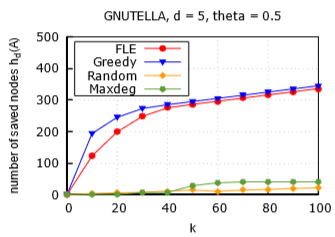
\includegraphics[height = 4.4cm]{picture/FLE/gnu_res} &
		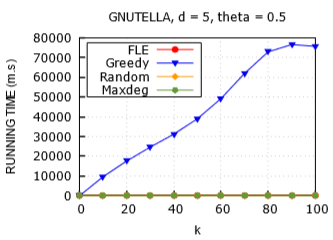
\includegraphics[height = 4.4cm]{picture/FLE/gnu_time} 
		\\
		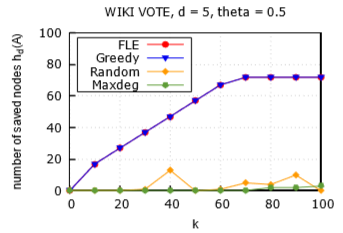
\includegraphics[height = 4.4cm]{picture/FLE/wiki_res} &
		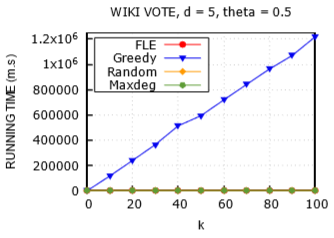
\includegraphics[height = 4.4cm]{picture/FLE/wiki_time} 
		\\
		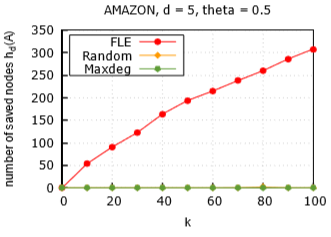
\includegraphics[height = 4.4cm]{picture/FLE/amazon_res} &
		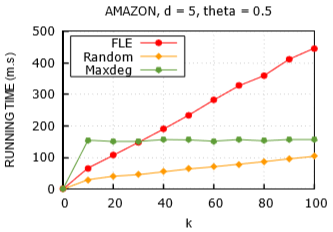
\includegraphics[height = 4.4cm]{picture/FLE/amazon_time} 
		\\
		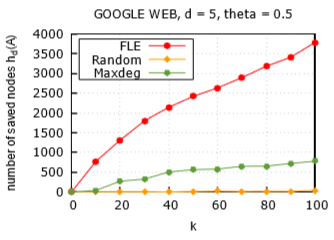
\includegraphics[height = 4.4cm]{picture/FLE/google_res} &
		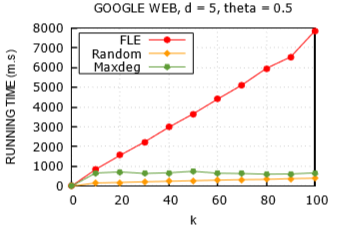
\includegraphics[height = 4.4cm]{picture/FLE/google_time} 
	\end{tabular}
	\caption{So sách chất lượng lời giải và thời gian chạy của các thuật toán khi $k$ thay đổi, $d=5$, $\theta=0.5$.} 
	\label{fig:FLE_k}   
\end{figure}

\begin{figure}
	\begin{tabular}{lll}
		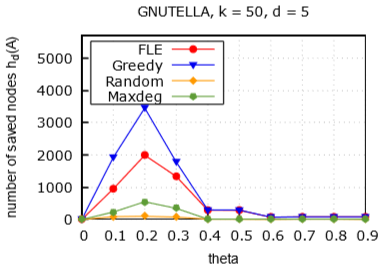
\includegraphics[height = 4.4cm]{picture/FLE/gnu_res_theta} &
		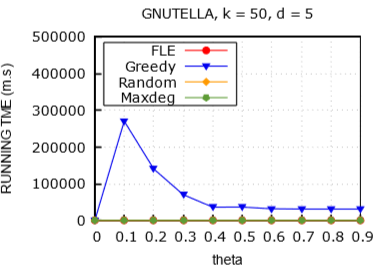
\includegraphics[height = 4.4cm]{picture/FLE/gnu_time_theta} 
		\\
		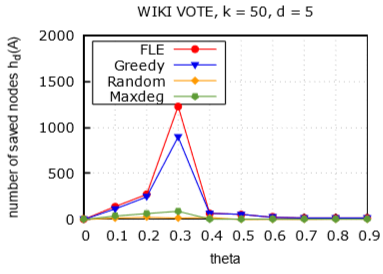
\includegraphics[height = 4.4cm]{picture/FLE/wiki_res_theta} &
		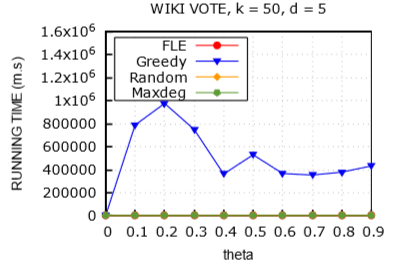
\includegraphics[height = 4.4cm]{picture/FLE/wiki_time_theta} 
		\\
		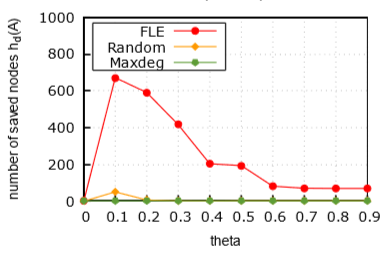
\includegraphics[height = 4.4cm]{picture/FLE/amazon_res_theta} &
		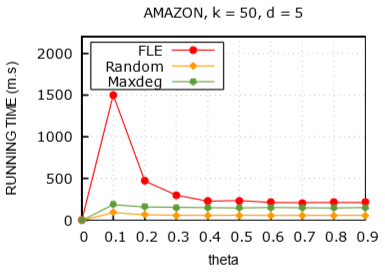
\includegraphics[height = 4.4cm]{picture/FLE/amazon_time_theta} 
		\\
		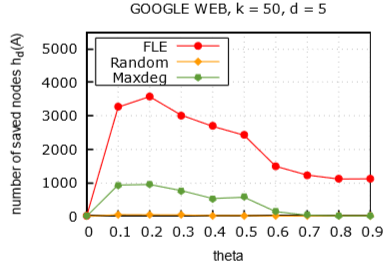
\includegraphics[height = 4.4cm]{picture/FLE/google_res_theta} &
		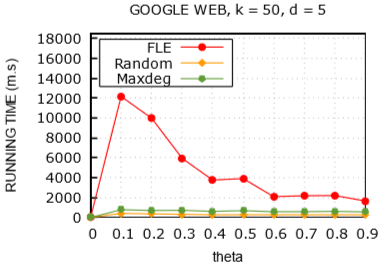
\includegraphics[height = 4.4cm]{picture/FLE/google_time_theta} 
	\end{tabular}
	\caption{So sách chất lượng lời giải và thời gian chạy của các thuật toán khi $\theta$ thay đổi, $d=5$, $k=50$.} 
	\label{fig:FLE_theta}   
\end{figure} 

\begin{figure}
	\begin{tabular}{lll}
		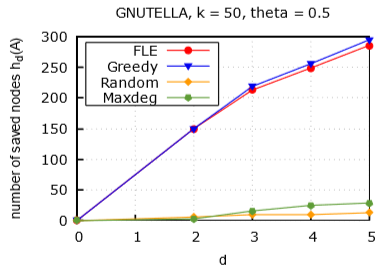
\includegraphics[height = 4.4cm]{picture/FLE/gnu_res_d} &
		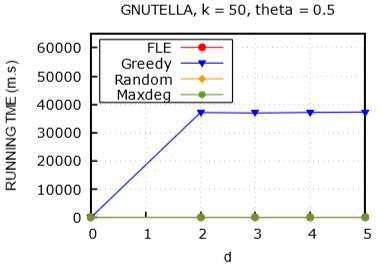
\includegraphics[height = 4.4cm]{picture/FLE/gnu_time_d}
	\end{tabular}
	\caption{So sách chất lượng lời giải và thời gian chạy của các thuật toán khi $d$ thay đổi, $\theta=0.5$, $k=50$ trong mạng Gnutella.} 
	\label{fig:FLE_d}   
\end{figure} 

\section{Giải pháp Targeted Misinformation Blocking (Xác định và ngăn chặn thông tin sai lệch trên mạng xã hội)}
{\itshape Dữ liệu có sẵn}	

Trong mục này chúng tôi đưa ra kết quả thực nghiệm của thuật toán STMB với 3 bộ dữ liệu và so sánh về chất lượng lời giải, tốc độ thực hiện với một số thuật toán cơ bản khác.

{\itshape - Dữ liệu:}
\begin{table}[h]
	\centering
	\begin{tabular}{|c|c|c|c|}
		\hline 
		Mạng & NetS \cite{NetS} & AS \cite{AS} & NetHEPT \cite{kemple1, chen10LT}\\ 
		\hline 
		Số đỉnh & 1.5K & 6.4K & 15.2K \\ 
		\hline 
		Số cạnh & 5.4K & 12.5K & 32.2K\\ 
		\hline 
		Bậc trung bình & 3.8 & 7.5 & 4.2\\ 
		\hline 
		Số đỉnh nguồn & 100 & 300 & 1000\\ 
		\hline 
	\end{tabular} 
	\caption{Các bộ dữ liệu dùng trong thực nghiệm với giải pháp TMB}
	\label{TMB:table}
\end{table}
Chúng tôi sử dụng 3 bộ dữ liệu mạng thực tế thu thập trên trang snap.stanford.edu \footnote{https://snap.stanford.edu/data/index.html}, thông tin về chúng được mô tả trong bảng \ref{TMB:table}. Theo các nghiên cứu trước \cite{khali, kemple1,chen10LT}, trọng số các cạnh của đồ thị trên mô hình LT được gán theo công thức $w(u,v) = 1/N_{in}(v)$. Với nguồn phát tán thông tin sai lệch chúng tôi chọn ngẫu nhiên từ 4-6\% số lượng đỉnh của cả đồ thị. Code được viết bằng ngôn ngữ Python 2.7, sử dụng thư viện hỗ trợ NetworkX và chạy trên máy Linux Server với 2.30 GHz Intel\textsuperscript{\textregistered} Xeon\textsuperscript{\textregistered} CPU E5-2697 and 128G of RAM DDR4. Trong thực nghiệm, chúng tôi so sánh thuật toán STMB với một số thuật toán khác được liệt kê dưới đây:
\begin {itemize}
\item PageRank: Tính toán ranking của các đỉnh trong đồ thị G dựa vào cấu trúc các cạnh liên kết với nó. Đây là thuật toán được thiết kế để xếp hạng các trang web từ đó đưa ra kết quả tìm kiếm. Do $h(\cdot)$ là hàm monotone nên sau khi sắp xếp hạng của các đỉnh trong đồ thị, chúng tôi sử dụng thuật toán tìm kiếm nhị phân để tìm kiếm tập lời giải A với |A| đỉnh có rank lớn nhất.
\item High-Degree: Một thuật toán heuristic dựa vào bậc của một đỉnh. Tương tự như thuật toán PageRank sau kho sắp xếp các đỉnh dựa trên bậc của chúng, chúng tôi sử dụng thuật toán tìm kiếm nhị phân để tìm lời giải cho bài toán.
\item Greedy: Thuật toán Greedy đưa ra trong thuật toán \ref{GA} kết hợp với các tối ưu trong \cite{Jleskovec}
\end{itemize} 

{\itshape - Kết quả thực nghiệm:} Như mô tả trong hình \ref{solSTMB}, số lượng đỉnh được chọn đưa ra bởi thuật toán STMB là nhỏ nhất. STMB tốt hơn lên đến 39\% so với thuật toán Greedy, hơn 60\%-95\% và 57\%-87\% so với thuật toán PageRank và High-Degree tương ứng. Để kiểm tra kết quả thu được từ thuật toán STMB, chúng tôi chạy 1000 mẫu Monte-Carlo để ước lượng giá trị của hàm $h(A)$ và kết quả kiểm tra được đưa ra trong hình \ref{checkSTMB}. Trong hầu hết các trường hợp $h(A)$ vượt qua ngưỡng yêu cầu.
\begin{figure}
\begin{tabular}{lll}
	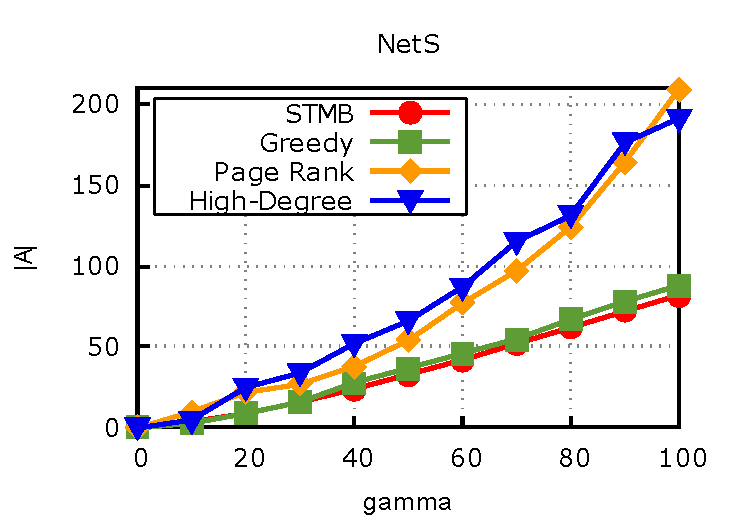
\includegraphics[height = 3.2cm]{picture/NetS} &
	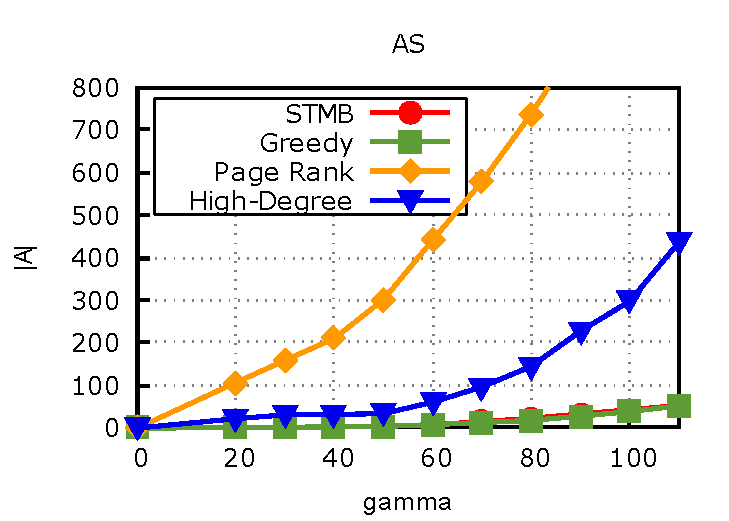
\includegraphics[height = 3.2cm]{picture/AS} &   
	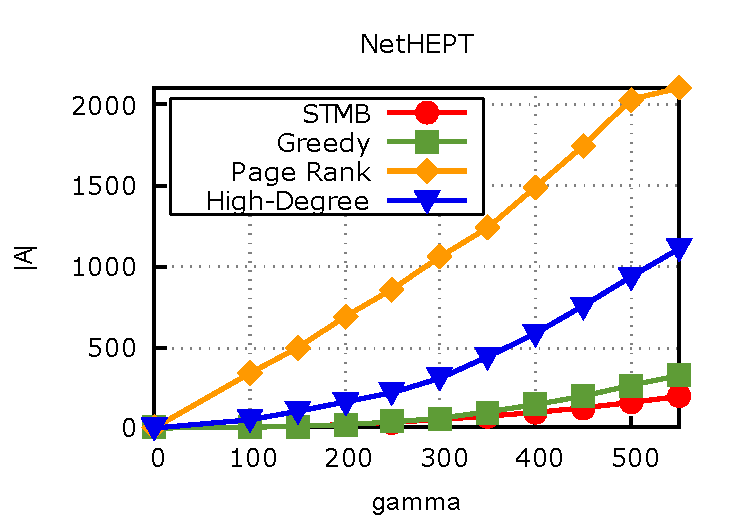
\includegraphics[height = 3.2cm]{picture/NetHEPT}
	\\
	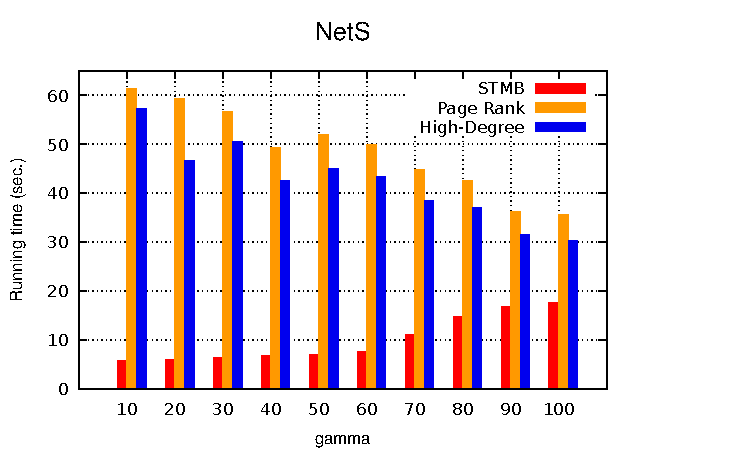
\includegraphics[height = 3.2cm]{picture/TimeNetS} &
	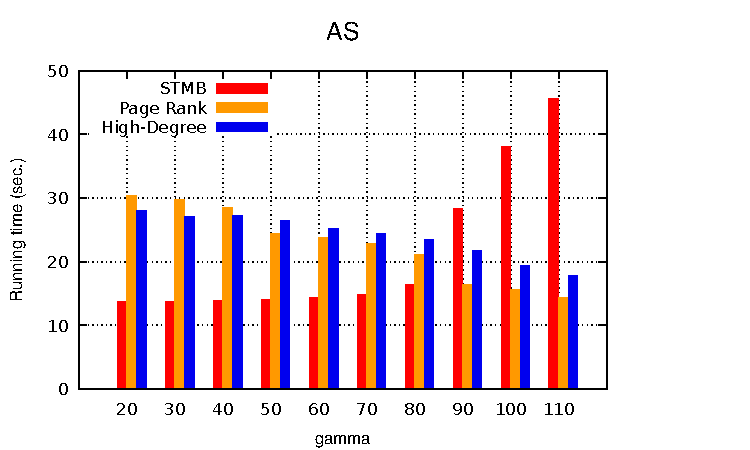
\includegraphics[height = 3.2cm]{picture/TimeAS} &   
	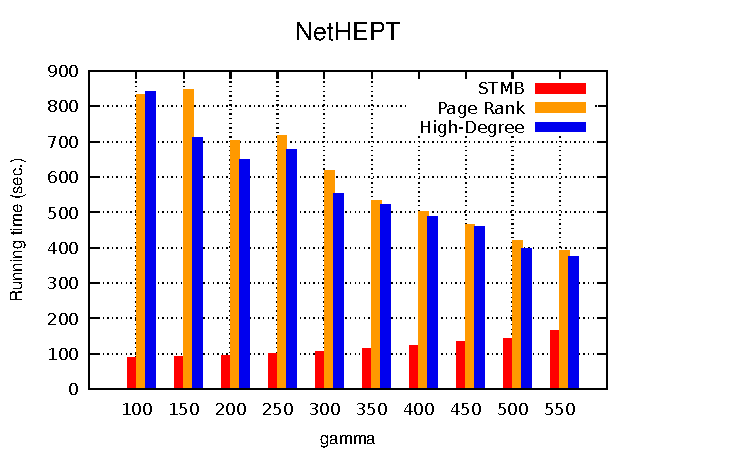
\includegraphics[height = 3.2cm]{picture/TimeNetHEPT}
\end{tabular}
\caption{So sách chất lượng lời giải và thời gian chạy của các thuật toán cho bài toán TMB}
\label{solSTMB}    
\end{figure}
\begin{figure}[htp]
\begin{tabular}{ccc}
	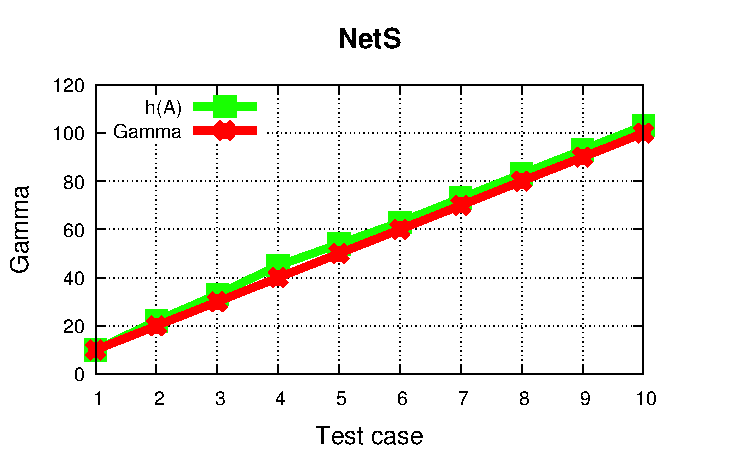
\includegraphics[height = 3.2 cm]{picture/CheckNetS} &
	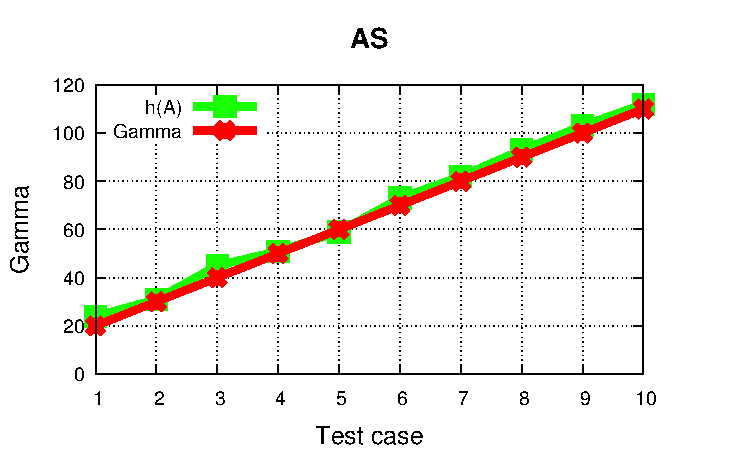
\includegraphics[height = 3.2 cm]{picture/CheckAS} &   
	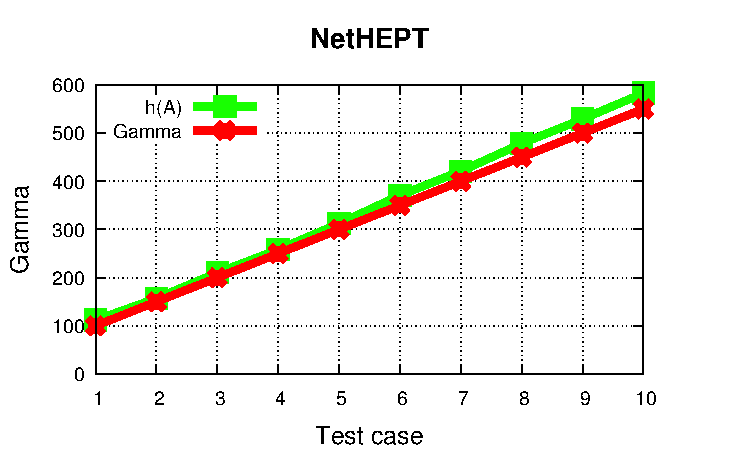
\includegraphics[height = 3.2 cm]{picture/CheckNetHEPT}
\end{tabular}
\caption{Kiểm tra kết quả của thuật toán STMB}
\label{check}    
\end{figure}

Thời gian chạy của các thuật toán trên 3 bộ dữ liệu trong trường hợp có $\gamma$ là lớn nhất được đưa ra trong bảng \ref{timeSTMB}. Ta thấy thuật toán Greedy có chất lượng lời giải tương đương với thuật toán STMB song thời gian thực nghiệm trên các bộ dữ liệu lại rất không hiệu quả.
\begin{table}[h]
\label{tab:time}       % Give a unique label
% For LaTeX tables use
\begin{center}
	\begin{tabular}{|c|c|c|c|c|}				
		\hline 
		\textbf{} & {$\mathsf{STMB}$} & {$\mathsf{Greedy}$} & {Page Rank} & {High-Degree} 				
		\\ 
		\hline 
		NetS & \textbf{17.57(s)} &	14206.80(s) &	35.73(s) &	30.24(s)
		\\ 
		\hline 
		AS & 45.70(s) & 14074.87(s) & \textbf{14.39(s)} &	17.85(s)
		\\
		\hline 
		NetHEPT & \textbf{165.12(s)} & 582566.74(s) & 392.34(s) & 374.66(s)
		\\
		\hline 
	\end{tabular}
\end{center}
\caption{So sánh thời gian chạy của các thuật toán với trường hợp $\gamma$ lớn nhất}
\end{table}



